\documentclass{article}

\usepackage{graphicx} % Required for inserting images
\renewcommand{\figurename}{Abbildung}
\usepackage{amsmath}
\usepackage{hyperref}

\title{Mein erstes LaTeX Dokument}
\author{Lennart Oelschläger}
\date{15.10.2024}

\begin{document}

\maketitle

\section{Mathematische Formeln}

\begin{enumerate}
    \item Formeln können so $f(x) = x^2$ eingegeben werden. 
    \item Umfangreichere Formeln können wir absetzen:
    $$ \exp(x) =  \lim_{n \to \infty} \left( 1 + \frac{1}{n} \right)^n $$
    \item Wir können solche Formeln auch nummerieren ...
    \begin{equation}
        \label{eq:exponential_function}
        \exp(x) = \sum_{n = 0}^\infty \frac{x^n}{n!}
    \end{equation}
    ... und später diese Formel mit \eqref{eq:exponential_function} referenzieren.
\end{enumerate}

\section{Auflistungen}

\subsection{Variante 1}

% Textformatierung
Die \textbf{jährlichen} \underline{Benzinkosten $C$} ergeben sich aus dem \textit{Produkt} des Preises $P$ pro Liter Benzin, der Benzinverbrauch $V$ in Liter pro Kilometer und der Kilometeranzahl $K$ pro Jahr.

\subsection{Variante 2}

Die jährlichen Benzinkosten ergeben sich aus $$ C = P \cdot L \cdot K, $$ wobei

\begin{itemize}
    \item $C$ die jährlichen Benzinkosten,
    \item $P$ den Preis pro Liter Benzin,
    \item $V$ den Benzinverbrauch in Liter pro Kilometer und
    \item $K$ die Kilometerzahl pro Jahr bezeichnet.
\end{itemize}

\section{Grafiken}

Grafiken können mithilfe der \texttt{figure}-Umgebung beschriftet und referenziert werden:

\begin{figure}[ht] % oder t, falls Grafiken immer oben ("top") erscheinen sollen
    \centering
    % benötigt \usepackage{graphicx} in der Präambel
    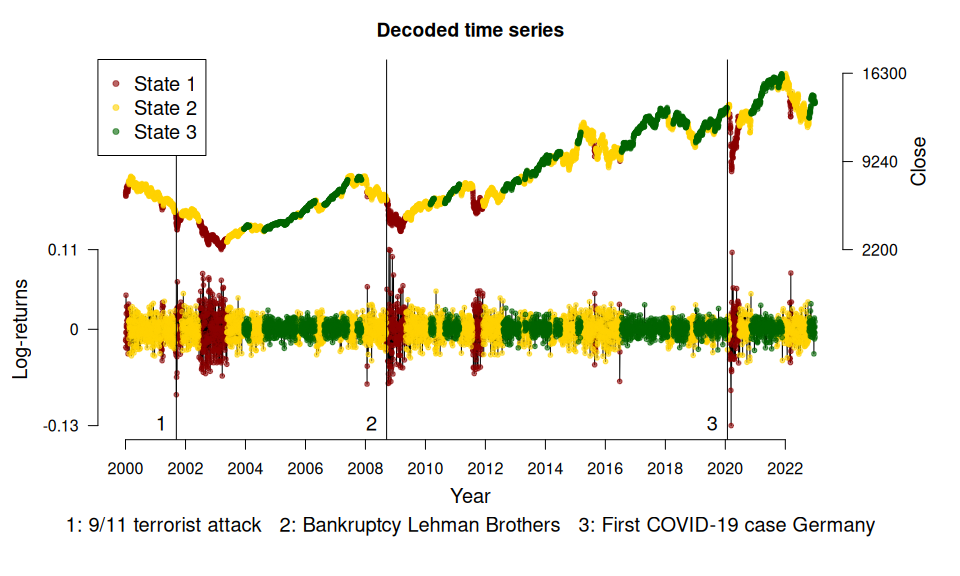
\includegraphics[width = \textwidth]{time_series.png}
    % mit in \renewcommand{\figurename}{Abbildung} zu "Abbildung" umbenennen
    \caption{Der Verlauf des DAX}
    \label{fig:dax}
\end{figure}

Abbildung \ref{fig:dax} zeigt den Verlauf des Deutschen Aktienindex (DAX). Er wurde mithilfe eines Hidden Markov Models (HHM) dekodiert.

\end{document}